\documentclass[paper=letter, fontsize=14pt]{scrartcl} 


\usepackage[utf8]{inputenc}
\usepackage{color}
\usepackage{graphicx}
\usepackage{epsfig}
\usepackage{multirow}
\usepackage{colortbl}
\usepackage[table]{xcolor}
\usepackage{fancyhdr}
\usepackage{graphicx}
\usepackage{graphicx}
\usepackage{verbatim}
\usepackage{pictex}  
\usepackage{multimedia}
\usepackage{listings}
\usepackage{vmargin}
\usepackage{xcolor,colortbl}
\usepackage[spanish]{babel} % language/hyphenation
\usepackage{amsmath,amsfonts,amsthm} % Math packages
\usepackage{amsbsy}
\usepackage{amssymb}
\usepackage{fancyvrb}
\usepackage{sectsty} % Allows customizing section commands
\allsectionsfont{\centering \normalfont\scshape} % Make all sections centered, the default font and small caps

\usepackage{fancyhdr} % Custom headers and footers
\pagestyle{fancyplain} % Makes all pages in the document conform to the custom headers and footers
\fancyhead{} % No page header - if you want one, create it in the same way as the footers below
\fancyfoot[L]{} % Empty left footer
\fancyfoot[C]{} % Empty center footer
\fancyfoot[R]{\thepage} % Page numbering for right footer
\renewcommand{\headrulewidth}{0pt} % Remove header underlines
\renewcommand{\footrulewidth}{0pt} % Remove footer underlines
\setlength{\headheight}{13.6pt} % Customize the height of the header

\numberwithin{equation}{section} % Number equations within sections (i.e. 1.1, 1.2, 2.1, 2.2 instead of 1, 2, 3, 4)
\numberwithin{figure}{section} % Number figures within sections (i.e. 1.1, 1.2, 2.1, 2.2 instead of 1, 2, 3, 4)
\numberwithin{table}{section} % Number tables within sections (i.e. 1.1, 1.2, 2.1, 2.2 instead of 1, 2, 3, 4)
\setpapersize{A4}
\setmargins{2.5cm}       % margen izquierdo
{2.4cm}                        % margen superior
{16.5cm}                      % anchura del texto
{23.42cm}                    % altura del texto
{10pt}                           % altura de los encabezados
{1cm}                           % espacio entre el texto y los encabezados
{0pt}                             % altura del pie de página
{2cm}                           % espacio entre el texto y el pie de página

\setlength\parindent{0pt} % Removes all indentation from paragraphs - comment this line for an assignment with lots of text

\newcommand{\horrule}[1]{\rule{\linewidth}{#1}} % Create horizontal rule command with 1 argument of height

\title{	
\normalfont \normalsize 
\textsc{Centro de Investigaci\'on en Matem\'aticas (CIMAT). Unidad Monterrey} 
\\ [25pt] 
\horrule{0.5pt} \\[0.4cm] % Thin top horizontal rule
\huge \textbf{Solución aproximada de factores para el modelo APT}\\ 
\horrule{2pt} \\[0.5cm] % Thick bottom horizontal rule
}

\author{Ricardo Cruz} % Your name

\date{\normalsize\today} % Today's date or a custom date


\rhead{\begin{picture}(0,0) \put(-56.7,-50){
\includegraphics[width=20mm]{cimat.png}} \end{picture}}
\renewcommand{\headrulewidth}{0.5pt}

\pagestyle{fancy}

\begin{document}
\lstdefinestyle{customc}{
  belowcaptionskip=1\baselineskip,
  basicstyle=\footnotesize, 
  frame=lrtb,
  breaklines=true,
  %frame=L,
  %xleftmargin=\parindent,
  language=C,
  showstringspaces=false,
  basicstyle=\footnotesize\ttfamily,
  keywordstyle=\bfseries\color{green!40!black},
  commentstyle=\itshape\color{red!40!black},
  identifierstyle=\color{blue},
  stringstyle=\color{purple},
}

\lstset{breakatwhitespace=true,
  basicstyle=\footnotesize, 
  commentstyle=\color{green},
  keywordstyle=\color{blue},
  stringstyle=\color{purple},
  language=C++,
  columns=fullflexible,
  keepspaces=true,
  breaklines=true,
  tabsize=3, 
  showstringspaces=false,
  extendedchars=true}

\lstset{ %
  language=R,    
  basicstyle=\footnotesize, 
  numbers=left,             
  numberstyle=\tiny\color{gray}, 
  stepnumber=1,              
  numbersep=5pt,             
  backgroundcolor=\color{white},
  showspaces=false,             
  showstringspaces=false,       
  showtabs=false,               
  frame=single,                 
  rulecolor=\color{black},      
  tabsize=2,                  
  captionpos=b,               
  breaklines=true,            
  breakatwhitespace=false,    
  title=\lstname,             
  keywordstyle=\color{blue},  
  commentstyle=\color{dkgreen},
  stringstyle=\color{mauve},   
  escapeinside={\%*}{*)},      
  morekeywords={*,...}         
} 


\maketitle % Print the title


\pagebreak


La teoría de arbitraje, sugiere un modelo para el retorno esperado de un activo financiero, el cual es una función lineal de diversos factores macroeconómicos. Este modelo arroja el valor esperado de retorno de un activo y se toman decisiones de posiciones sobre los activos a partir de la comparación del resultado del modelo y el valor real.\\

La forma en que se plantea dicho modelo sugiere emplear la técnica de análisis de factores, pues cada retorno de un activo será una función lineal de los factores comunes.\\

Sin embargo, el análisis de factores arroja los factores salvo una rotación, la cual puede ser una tarea complicada de realizar. Es por eso que se opta por la solución aproximada de factores mediante el análisis de componentes principales.\\

Si se considera un portafolio con $p$ activos, observados durante $n$ periodos, entonces, el modelo para el retorno esperado con $k$ factores es:

$$R=LF'+\epsilon$$

Donde $R$ es la matriz de retornos con dimensión $p\times n$. $F$ es la matriz de factores comunes con dimensión $n \times k$. $L$ es la matriz de pesos con dimensión $p\times k$ y $\epsilon$ es la matriz de ruido con dimensión $p\times n$ \\

Para este modelo, la matriz de covarianza del modelo esta dada por $\Sigma=\sigma_f^2LL'+\sigma_\epsilon^2\mathbb{I}_p$

Los valores propios para esta matriz están dados por:

\begin{eqnarray*}
\lambda_1&=&\sigma_f^2(b^2pk+p\sigma_b^2)+\sigma_\epsilon^2\\
\lambda_i&=&\sigma_f^2\sigma_b^2+\sigma_\epsilon^2 \hspace{1cm} i=2,\hdots,k\\
\lambda_i&=&\sigma_\epsilon^2 \hspace{1cm} i=k+1,\hdots,p\\
\end{eqnarray*}


La aproximación se realizará mediante simulación, tomando $b=1,\sigma_b^2=0.01,sigma_f^2=0.000158,\sigma_\epsilon^2=0.0045$. Con $n=80, k=4$ y variando el número de activos $p$ entre 50 y 100\\

La figura \ref{f1}, muestra 100 simulaciónes de los eigenvalores de $\Sigma$, esto se realizó simulando las matrices $L,F,\epsilon$, en donde cada una de las entradas de las matrices sigue la distribución $N(b,\sigma_b^2)$, $N(0,\sigma_f^2)$ y $N(b,\sigma_\epsilon^2)$ respectivamente.\\

Posterior a simular las matrices, se calcula $R$ y $\Sigma=\dfrac{RR'}{n}$, de donde se obtienen los eigenvalores.\\

\begin{figure}
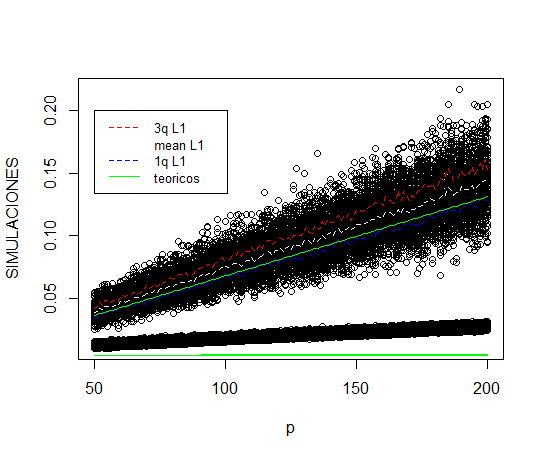
\includegraphics[scale=1]{Rplot.png} 
\label{f1}
\end{figure}

Se observa como para el primer valor propio, el valor teórico esta por debajo de la media y se acerca más al primer cuantíl. De forma similar, los valores teóricos de los siguientes 4 valores propios se encuentran por debajo de los observados en la simulación. Este comportamiento se hace más notable conforme el número de activos crece.\\

Podría decirse que esto se debe a la calidad de la simulación de las matrices que definene a $R$, además de ser una aproximación y está implícito un error respecto al valor real.\\

También puede observarse, que el primer valor propio es significativamente más grande que el resto de eigenvalues.

\end{document}